\section[Program Costs of ABC/CARE]{Program Costs\footnote{Sylvi Kuperman greatly assisted us in preparing this section of the appendix.}} \label{app:programcosts}

\noindent In this appendix, we document the sources informing our programs' costs calculation in Section~\ref{section:programscosts}. We use a battery of primary sources obtained in the Archives of the University of North Carolina at Chapel Hill---Records of the Office of the Vice Chancellor \citet{UNC-Archives_Health-Affairs}. Figure~\ref{figure:who} exemplifies one of these sources, in which the monthly cost of treatment per child for the year 1977 is categorized by source of funding.

\begin{center}
\begin{figure}[H] 
\caption{Primary-source Document Costs, Example}
\label{figure:who}
\centering
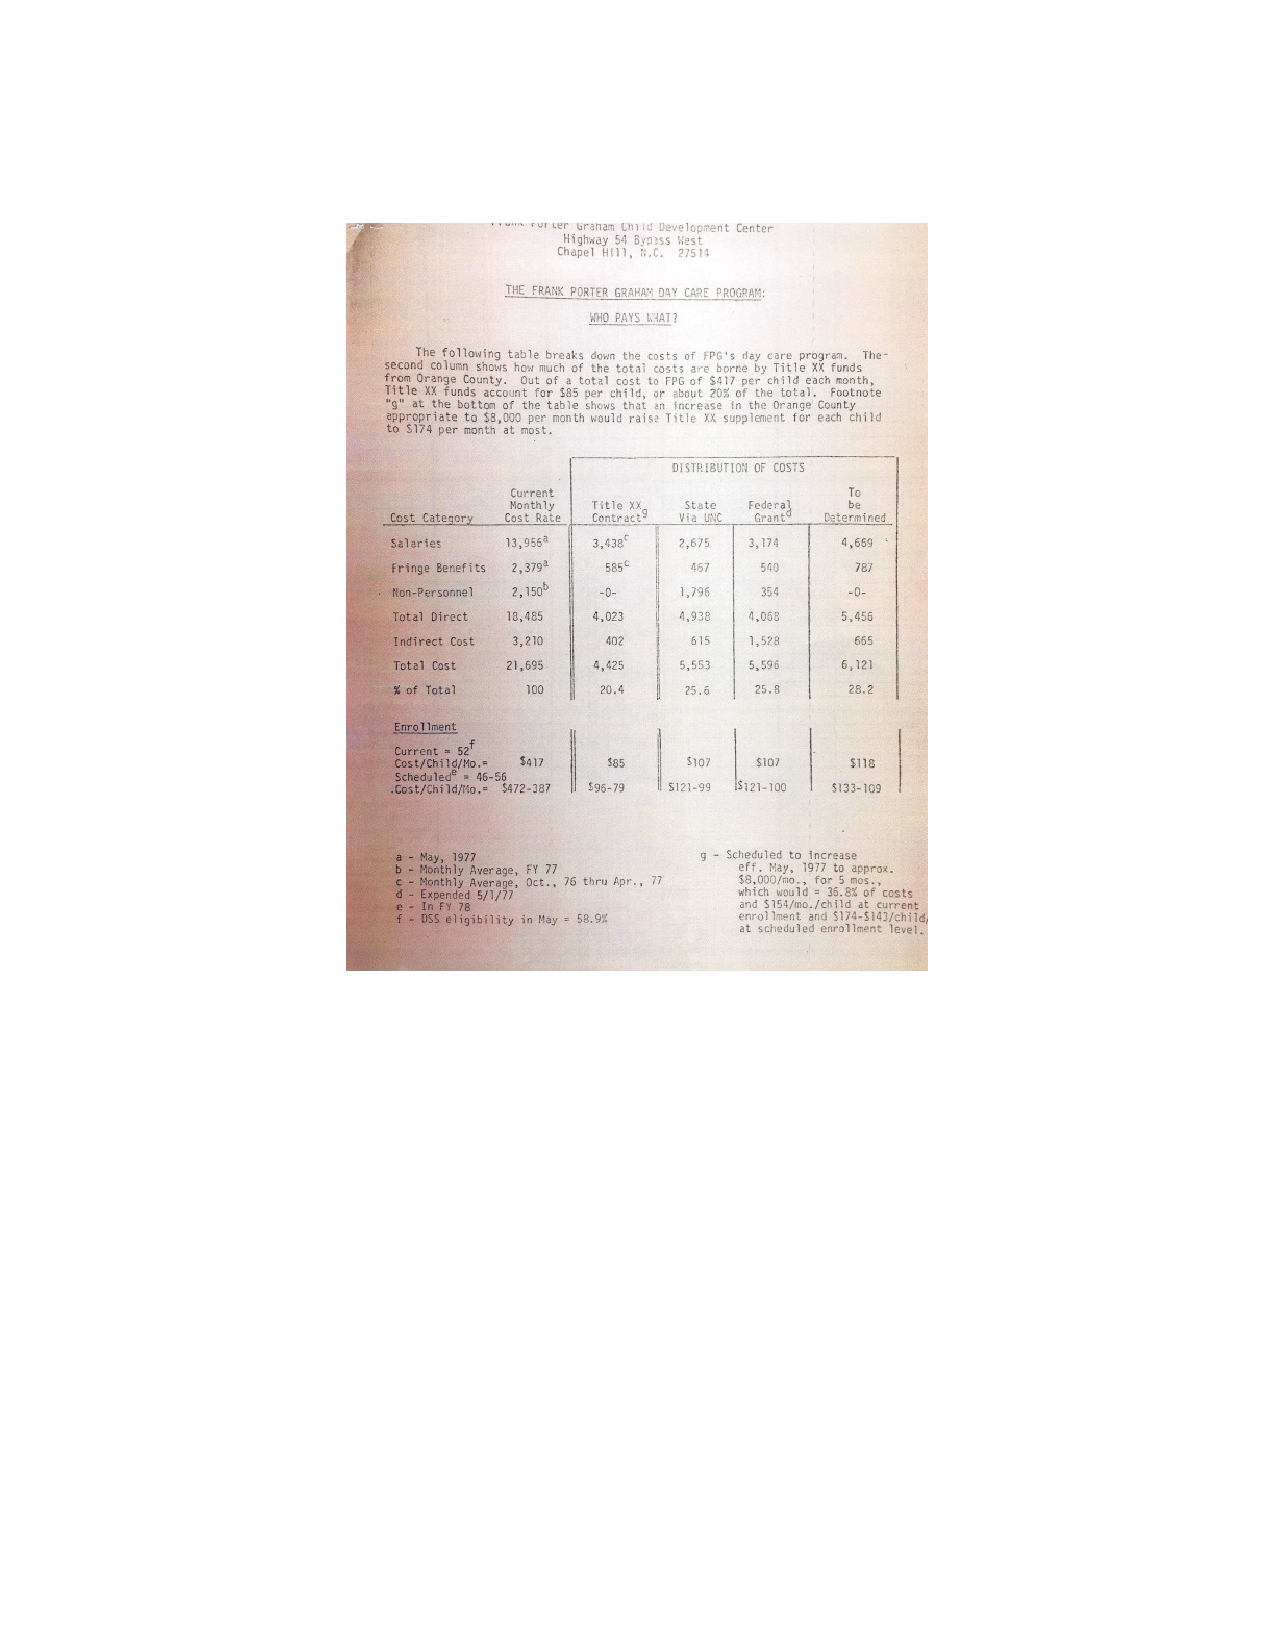
\includegraphics[width=.9\columnwidth]{AppOutput/Program/UNC-costs.pdf}
\floatfoot{
\footnotesize
Note: This figure is a photograph exemplifying the primary-source document we use in the calculation of the programs' cost. It was obtained in the University of North Carolina at Chapel Hill---Records of the Office of the Vice Chancellor}
\end{figure}
\end{center}

\noindent Figure~\ref{figure:wages} is another of our sources and it is the base of our calculation of personnel costs.

\begin{center}
\begin{figure}[H] 
\caption{Primary-source Document Costs, Personnel Wages}
\label{figure:wages}
\centering
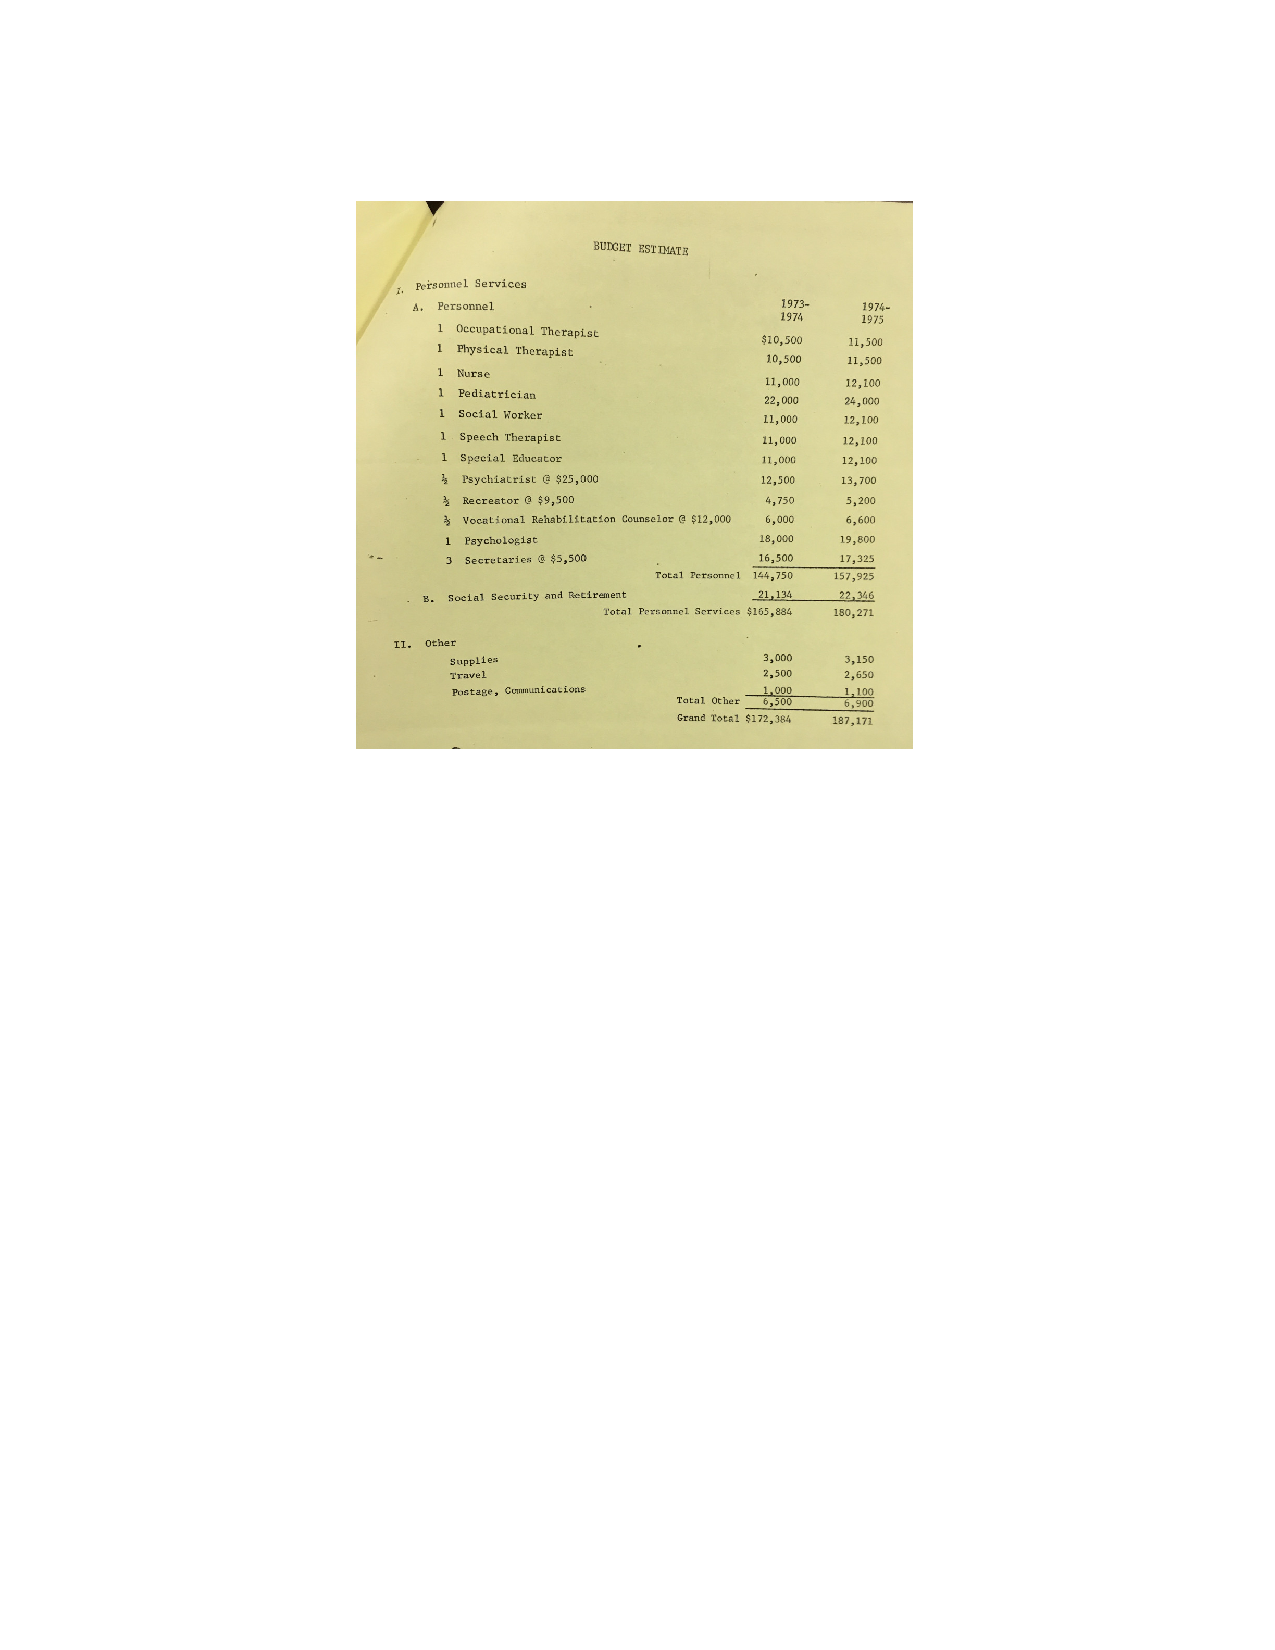
\includegraphics[width=.9\columnwidth]{AppOutput/Program/UNC-costs_budget.pdf}
\floatfoot{
\footnotesize
Note: This figure is a photograph provides the estimates for the personnel wages we use. It was obtained in the University of North Carolina at Chapel Hill---Records of the Office of the Vice Chancellor}
\end{figure}
\end{center}

\noindent Interviews with the programs' staff \citet{projectcare2014interviews,abc2014-2015interviews}, inform us about additional costs of the programs. An example is the salary of a social worker, who is not part of some of the of the costs estimates reported before but was part of the staff implementing treatment. These interviews are available upon request.\\ 

\noindent Finally, a valuable source is a report written by the program staff \citet{FPG_1979_Progress-Report}. As we note in Section~\ref{section:programscosts}, this report produced an estimate of the cost in a completely independent way, although perhaps using the same or similar primary sources. Our calculation of the costs comes very close to those in \citet{FPG_1979_Progress-Report}. \\

\noindent We summarize the yearly program costs of ABC/CARE in Table~\ref{tab:totalcosts}. \\

\begin{table}[H]
\centering
\begin{threeparttable}
\caption{Yearly Program Costs, ABC/CARE} \label{tab:totalcosts}
\footnotesize
\begin{tabular}{lc} \toprule
\multicolumn{1}{c}{Item} & Yearly Cost in 2014 USD \\ \midrule
1 Program Director & $60,935$ \\ 
1 Social Worker      &  $35,869$ \\ 
3 Lead Teachers and 2 Teachers Aides (Nursery)  & $204,457$ \\
4 Lead Teachers and 4 Teacher Aides  (Toddlers) & $305,181$ \\ 
2 Teaching Support Staff & $53,341$ \\ 
1 Secretary & $32,973$ \\ 
1 Clerk        & $32,537$ \\ 
Workers' Fringe Benefits & $124,935$ \\ 
Other & $4, 891$ \\ \\ \midrule 
Total  & $962,726$ \\ 
Total per Subject & $18,514$ \\ \bottomrule
\end{tabular}
\begin{tablenotes}
\footnotesize
\item Note: This table summarizes the yearly costs for ABC/CARE. They are based on primary-source documentation describing ABC. We assume that the costs for ABC and CARE were the same based on conversations with programs' staff \citep{projectcare2014interviews,abc2014-2015interviews}. \\
\end{tablenotes}
\end{threeparttable}
\end{table}